\section{Task 3}
\FloatBarrier % Now figures cannot float above section title

Here are the drawing of the kinematic diagram using the Denevit-Hartenberg frame rules for the robot designed in task 1.

\begin{figure}[htbp]
    \centering
    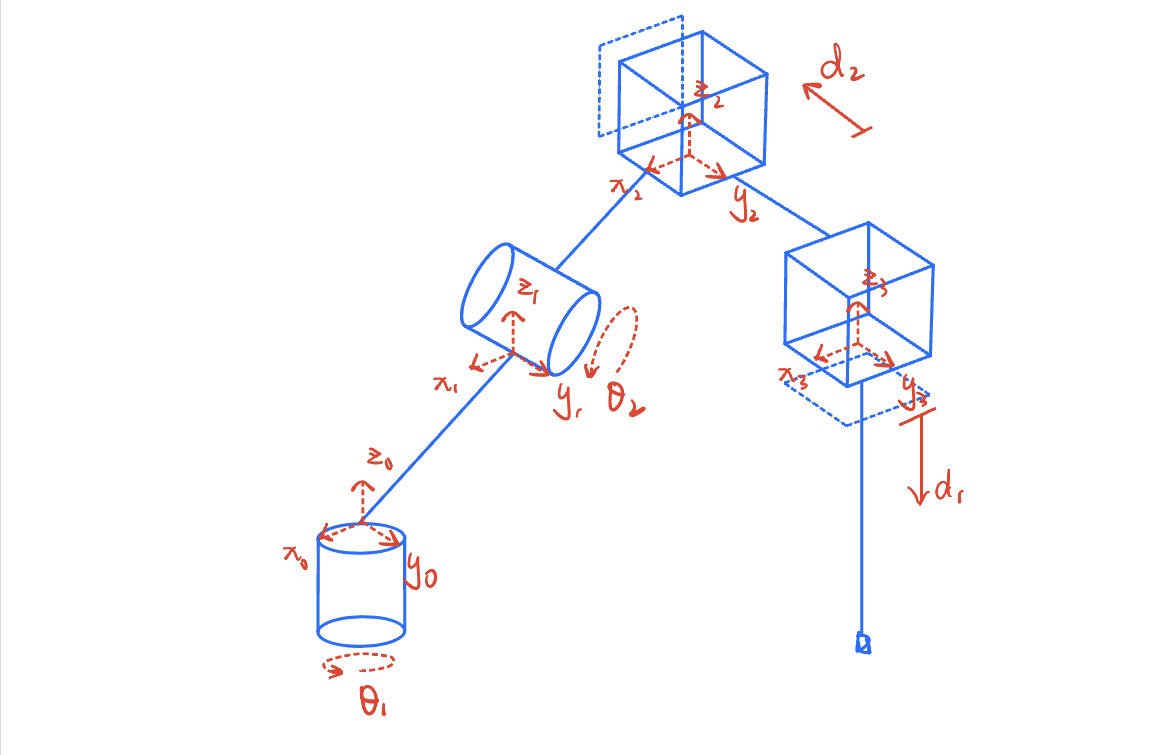
\includegraphics[width=10cm]{./fig/D-H.jpg}
    \caption{Experimental results}
    \label{f5}
\end{figure}



\iffalse
\subsection*{A : presentation of force vs deformation relationships}
Using the data in Table 2, the force vs deformation plot can be derived as \autoref{f3}. Also, from the lecture in week 7, we can learn that the total bending moment diagram is as follows


\begin{figure}[htbp]
    \centering
    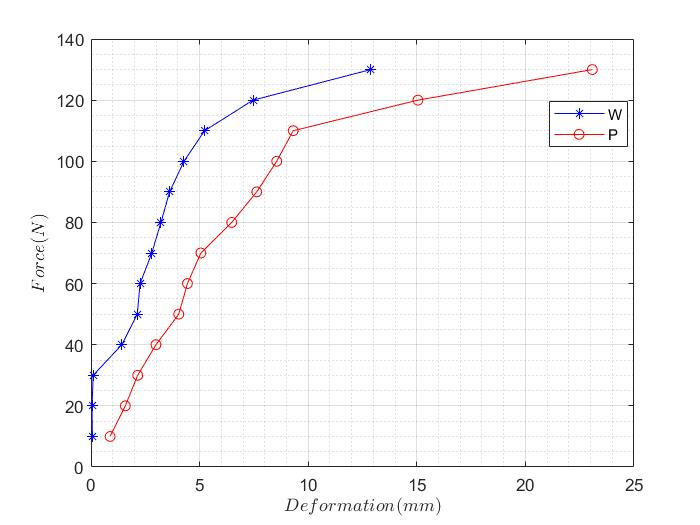
\includegraphics[width=9cm]{./fig/17.jpg}
    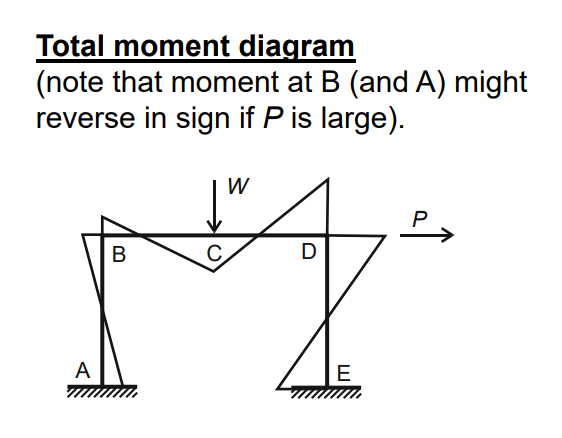
\includegraphics[width=7cm]{./fig/16.png}
    \caption{Force vs deformation and total moment diagram}
    \label{f4}
\end{figure}


The chart illustrates the relationship between the strength and deformation of steel, which can be discussed in two different situation.

$\bullet$ W<110N,P<110N: Elastic deformation: The relationship between the elastic deformation variable and the external force is linear.

$\bullet$ W$\geq$110N,P$\geq$110N: Plastic deformation: The relationship between force and deformation is nonlinear, i.e., the strain shows a rapid increase with the increase of stress.

From the overall bending moment diagram (see \autoref{f4}), it can be seen that point D has the maximum bending moment, making it the first point in the experiment to experience plastic deformation.

In \autoref{f3}, The P-W graph is piecewise and if the combination of the P and W exceeds the closed figure on the left, The collapse will happen. In this case$(y=x)$, the collapse load for the frame was $W=148.63N,P=148.63N(Theoretical)$.

Based on the \autoref{f4} (ignoring the inaccurate data at the beginning), it can be analyzed that the first plastic hinge is formed at around 110 N, where a significant change can be observed in the slope of the W curve. The remaining plastic hinges are formed at around 120 N, where both the P and W segments exhibit drastic changes.

%\textit{Can you identify at which load each plastic hinge formed?}


\subsection*{B : explaination of plastic hinges}

\begin{figure}[htbp]
    \centering
    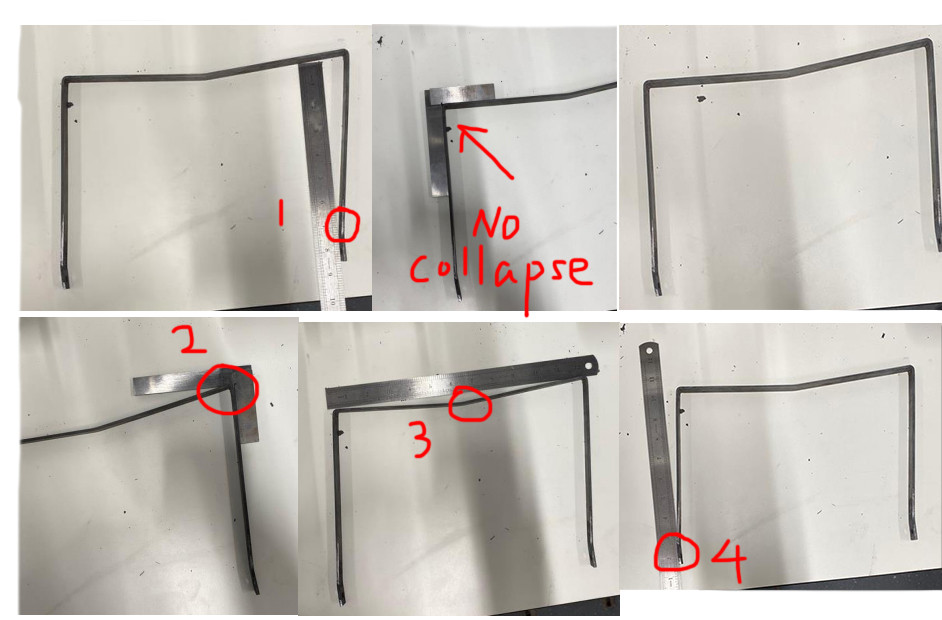
\includegraphics[width=10cm]{./fig/18.jpg}
    \caption{Experimental results}
    \label{f5}
\end{figure}

There are 4 plastic hinges at the moment of the collapse of the frame. Compare \autoref{f2} and \autoref{f5} we can find: 

$\bullet$ After the force load, the upper left corner of the frame did not rotate, and the angle between the beam and column was still degrees.

$\bullet$ The angle of rotation of the plastic collapse occurring at points 1,4 is $\theta$(in \autoref{f2}).

$\bullet$ The angle of rotation of the plastic collapse occurring at points 2,3 is $2\theta$(in \autoref{f2}), which is double that of points 1,4.

\subsection*{C : compare the theoretical and actual}
\subsubsection*{i}

The theoretical plastic collapse load derived from Section 2 is 148.63N, while the actual collapse load is in the region of $110N$-$120N$.($23.8\%$)

The comparison leads to the conclusion that the actual collapse load will be less than the theoretical value for these possible reasons:

$\bullet$ \textbf{Geometric discrepancies:} The actual dimensions of the frame may differ from the theoretical dimensions, as seen in \autoref{t1}. These discrepancies may affect the frame's overall stiffness and load-carrying capacity.(theoretical $M_p=6.75N$ vs actual $M_p=8.67N$)

$\bullet$ \textbf{Material imperfections:} The mild steel used in the experiment may contain imperfections like inclusions, voids, or uneven distribution of constituents, which could affect its mechanical properties and reduce its strength.

$\bullet$ \textbf{Load application:} The loading rig's accuracy in applying the horizontal and vertical loads may impact the results. Inaccurate load distribution or misalignment could cause the frame to experience additional stresses, leading to a reduced collapse load.

$\bullet$ \textbf{Measurement errors:} The gauges used to monitor the deflection of the frame might have inaccuracies, leading to discrepancies between the actual and recorded deflections.

\subsubsection*{ii}

$\bullet$ There are 4 plastic hinges in theory (\autoref{f2}-Combined mechanism). The positions of the plastic hinges are points A, C, D and E.

$\bullet$ There are 4 plastic hinges in experiment (\autoref{f5}). The positions of the plastic hinges are in the position 1,2,3,4.

$\bullet$ Compared with that, it is easy to see that the theoretical and actual positions of the plastic hinges are roughly the same.

\subsubsection*{iii}

The overall shape of the measured and predicted collapse mechanism are same. In \autoref{f2} and \autoref{f5}, the upper left corner is not deformed, a rotation of angle $\theta$ occurs at positions 1,4 and a rotation of angle $2\theta$ occurs at positions 2,3.
\fi